%/////////////////////////////////////////////////
%/
\chapter{Preliminaries}
%/
%/////////////////////////////////////////////////
\label{chap:Preliminaries}
%/////////////////////////////////////////////////
%/
\section{Propositional Logic}
%/
%/////////////////////////////////////////////////
\label{sec:PropositionalLogic}
% checked
Propositional logic deals with logical relationships between propositions.
A proposition is a boolean variable that has either a truth value $\mathit{true}$ or a truth value $\mathit{false}$, also called atomic proposition.
The syntax of well-formed propositional formulas:\newline

\begin{table}[!ht]
\centering
\begin{tabular}{lllllll}
$\mathit{\varphi}$ & := & $\mathit{a}$ & | & $\neg \mathit{\varphi}$ & | & $( \mathit{\varphi} \wedge \mathit{\varphi} )$
\end{tabular}
\end{table}

\noindent where $\mathit{a}$ is an atomic proposition.
So, a propositional formula can be an atomic proposition.
Also, propositional formulas can be constructed from atomic propositions by using logical connectives $\neg$ and $\wedge$.
There are some more logical connectives used in propositional logic, but they all are syntactic sugar.
In the syntax, we have only $\neg$ and $\wedge$ as logical connectives because these are sufficient to express syntactic sugar.
Syntactic sugar are:\newline

\begin{table}[!ht]
\centering
\begin{tabular}{ccc}
$\bot$                   & := & $( \mathit{a} \wedge \neg \mathit{a} )$ \\
$\top$                   & := & $( \mathit{a} \vee \neg \mathit{a} )$  \\
$( \mathit{\varphi_{1}} \vee \mathit{\varphi_{2}}$      & := & $\neg ( \neg \mathit{\varphi_{1}} \wedge \neg \mathit{\varphi_{2}} )$     \\
$( \mathit{\varphi_{1}} \to \mathit{\varphi_{2}} )$ & := & $( \mathit{\neg \varphi_{1}} \vee \mathit{\varphi_{2}} )$     \\
$( \mathit{\varphi_{1}} \Leftrightarrow \mathit{\varphi_{2}} )$       & := & $( \mathit{\varphi_{1}} \to \mathit{\varphi_{2}} ) \wedge ( \mathit{\varphi_{2}} \to \mathit{\varphi_{1}} )$     \\
$( \mathit{\varphi_{1}} \oplus \mathit{\varphi_{2}} )$      & := & $( \varphi_{1} \Leftrightarrow \neg \varphi_{2} )$     
\end{tabular}
\end{table}

\begin{example}
	Some propositional formulas are:
	$$\neg \mathit{a}$$
	$$ ( \neg \mathit{a} \wedge \underbrace{ ( \mathit{b} \vee \mathit{c} ) }\limits_{\mathit{\varphi_{1}}} ) $$
	$$ ( \mathit{b} \to \underbrace{ ( \mathit{a} \wedge \mathit{c} ) }\limits_{\mathit{\varphi_{2}}} ) $$
	Here,  $\mathit{a}$, $\mathit{b}$ and $\mathit{c}$ are atomic propositions, whereas $\mathit{\varphi_{1}}$ and $\mathit{\varphi_{2}}$ are propositional formulas.
\end{example}
%/////////////////////////////////////////////////
%/
\section{First-Order Logic}
%/
%/////////////////////////////////////////////////
\label{sec:FOLogic}
% checked
Propositional logic is simple. 
If we have propositions, we can build boolean combinations of them by just conjunction and negation.
This logic is not very expressive as propositional logic represents only facts.
So, sometimes propositional logic is not enough for modeling and we need a more expressive language.
By first-order (FO) logic, we can formalize a statement to a logic.\newline

\noindent FO logic represents facts, objects, and relations.
FO logic is a framework which has the ingredients, theory symbols, predicate symbols, and logical symbols.\newline

\noindent Theory symbols can be constants, variables, function symbols.
All constants and variables are terms.
If $t_{1}, \ldots, t_{n}$ are terms and $f$ is an $n$-ary funtion symbol, then $f(t_{1}, \ldots, t_{n})$ is also a term.
So, function symbols operate terms.
The difference between predicate symbols and function symbols is that the predicate symbols always give boolean values, but the function symbols give values from a domain.
Predicate symbols are special function symbols, but they have boolean values, and they made the switch from terms to boolean predicates.
If $t_{1}, \ldots, t_{n}$ are terms and $P$ is an $n$-ary predicate symbol $P(t_{1}, \ldots, t_{n})$ is called a constraint.
Logical symbols are logical connectives $\neg, \wedge, \vee, \to, \ldots$ and quantifiers.
Two types of quantifiers are available, existential quantifier ($\exists$) and universal quantifier ($\forall$).\newline

% checked
\noindent FO logic is called first-order logic because it allows the quantification over variables and it does not allow the quantification over predicates.
We can have a hierarchy of logic, for example, second-order logic, third-order logic and so on.
We are not going into the details of those as we are only interested in FO logic.\newline

\begin{example}
    Assume the following:
    \begin{itemize}
        \item All girls are cute.
        \item Lily is a girl.
        \item Therefore, Lily is cute.
    \end{itemize}
    We can formalize it by defining:
    \begin{itemize}
        \item Constants: $\hspace{13mm}$ Lily
        \item Variables: $\hspace{15mm} x$
        \item Predicate symbols: $\hspace{1mm}$ isGirl($\cdot$), isCute($\cdot$)
    \end{itemize}
    Formalization:
    \begin{itemize}
        \item $\forall x.$ isGirl($x$) $\to$ isCute($x$)
        \item isGirl($Lily$)
        \item isCute($Lily$)
    \end{itemize}
\end{example}

\noindent FO logic formulas can be constructed by the following syntax:
$$\varphi\hspace{5mm}:=\hspace{5mm}c\hspace{5mm}|\hspace{3mm}\neg\varphi\hspace{4mm}|\hspace{2mm}\varphi\wedge\varphi\hspace{2mm}|\hspace{5mm}\exists x.\varphi\hspace{2mm}|\hspace{5mm}\forall x.\varphi$$
Here, $c$ is a constraint.\newline

% checked
\begin{definition}
\label{def:Theory}
    (Theory).
    A theory $T$ is a set of sentences and the sentences are the formulas with non-logical symbols and no free variables defined in the following.
    TSat \cite{TSat}.
\end{definition}

\begin{definition}
\label{def:Free_Variables}
    (Free Variable).
    A variable is a free variable if it occurs in a formula and is not bound by a quantifier.
    For $\forall x. \varphi$ and $\exists x. \varphi$, we call $\varphi$ the scope of the quantification for $x$ and we call occurances of $x$ in $\varphi$ bounded.
\end{definition}

\begin{example}
    The following is a FO logic formula over the theory of integers with addition, also called linear integer arithmetic:
    $$  \forall x. \exists y. \hspace{2mm} (x + 1 < y) \hspace{2mm} \wedge  \hspace{2mm} (x + 2 = z) $$
    Here, $1$ and $2$ are constants, $x, y$ and $z$ are variables, $+$ is a function symbol, $<$ and $=$ are predicate symbols, $\wedge$ is a logical connective and $\forall$ and $\exists$ are quantifiers.
\end{example}
%/////////////////////////////////////////////////
%/
\subsection{Quantifier-Free FO Logic}
%/
%/////////////////////////////////////////////////
\label{subsec:Quantifire_Free_FO_Logic}
% checked
A quantifier-free formula in FO logic is a formula that does not contain quantifiers.
In other words, a quantifier-free formula is either a constraint which has truth values or the application of logical connectives to constraints.
So, quantifier-free FO logic formulas have the following syntax:
$$\varphi\hspace{5mm}:=\hspace{5mm}c\hspace{5mm}|\hspace{3mm}\neg\varphi\hspace{4mm}|\hspace{2mm}\varphi\wedge\varphi$$

\begin{example}
    An example quantifier-free FO logic formula for non-linear integer arithmetic including multiplication:
    $$ ((x + 1 < y) \hspace{2mm} \wedge  \hspace{2mm} (x + 2 = z))  \hspace{2mm} \vee \hspace{2mm} (x + 6 = yz) $$
\end{example}

\noindent If each constraint of a quantifier-free FO logic formula is replaced by boolean variables, we will have a boolean skeleton, and the formula will become a propositional logic formula.
Because in propositional logic we only need boolean variables as the logical connectives are already in quantifier-free FO logic.
Thus, propositional logic is also a FO logic.\newline

\begin{example}
    The followings are example for a quantifier-free FO logic formula $\varphi_{QF}$ and its boolean skeleton $\varphi_{sk}$ which is a propositional logic formula:
    \begin{table}[!ht]
    \centering
    \begin{tabular}{lcccccc}
    $\varphi_{QF}$ & := & $((x + 1 < y)$ & $\wedge$ & $(x + 2 = z))$ & $\vee$ & $(x + 6 = yz)$ \\
    $\varphi_{sk}$  & := & $(a$            & $\wedge$ & $b)$            & $\vee$ & $c$           
    \end{tabular}
    \end{table}
\end{example}
%/////////////////////////////////////////////////
%/
\section{Real Arithmetic}
%/
%/////////////////////////////////////////////////
\label{sec:Real_Arithmetic}
% checked
Real arithmetic (RA) is a first-order theory $(\mathbb{R}, +, \ast, 0, 1, <)$ over the reals with addition and multiplication. 
RA constraints can be built upon constants $0, 1$, real-valued variables $x$ and the functions addition $+$ and multiplication $\ast$ according to the following quantifier-free syntax:\newline

\begin{table}[!ht]
\begin{tabular}{lccccccccccc}
\centering
Terms:       & $t$       & := & $0$   & | & $1$            & | & $x$                          & | & $t+t$ & | & $t \ast t$ \\
Constraints: & $c$       & := & $t<t$ &   &                &   &                              &   &       &   &             \\
Formulas:    & $\varphi$ & := & $c$   & | & $\neg \varphi$ & | & ( $\varphi \wedge \varphi$ ) &   &       &   &           
\end{tabular}
\end{table}

% checked
\noindent A monomial is the product of variables, and the empty product represents the constant $1$. 
A constraint is a condition of a RA problem that the solution must satisfy.
We use $\mu$ to denote assignments (i.e., functions assigning values to all variables) and write $\mu (x)$ for the value of $x$ under $\mu$.
There are also syntactic sugar such as the relational operators $>, \leq, \geq, =, \neq$ and the logical connectives $\vee, \to$.
The semantics is defined as usual.\newline

\noindent Terms are also called polynomials.
In other words, a polynomial $p\in R[x]$ is a sum of terms, each term being a variable raised to a power and multiplied by a coefficient from some coefficient ring $R$.
If a polynomial has only one variable (i.e. its coefficient are variable-free), it is called univariate, else it is called multivariate: 
$$ p(x) = a_{d}x^{d} + a_{d-1}x^{d-1} + \ldots + a_{0}x^{0} $$
where $a_{0}, a_{1}, \ldots a_{d} \in R$ for some non-negative integer $d$.\newline

% checked
\noindent The degree of $x$ in a monomial is the exponent of $x$, and the total degree of the monomial is the sum of the degree of each variable appearing in that monomial.
The degree of $x$ in the polynomial $p$ is the maximal $0\leq k\leq d$ such that $a_{k}\neq 0$ whereas the total degree of $p$ is the maximal degree among its monomials.\newline
A monomial is linear if it has total degree less than or equal to one. 
Otherwise, it is nonlinear and similarly for polynomials.\newline

\noindent Formulas without multiplication form the logic of linear real arithmetic (LRA).
When multiplication is allowed we call RA non-linear real arithmetic (NRA).\newline

\noindent Please note that in this thesis work we will be dealing with quantifier-free LRA and NRA.
So, from now on if we use the word LRA and NRA, that means we are talking about quantifier-free LRA and NRA.
%/////////////////////////////////////////////////
%/
\subsection{Linear Real Arithmetic}
%/
%/////////////////////////////////////////////////
\label{subsec:LRA}
% checked
Linear real arithmetic is a first-order theory $(\mathbb{R}, +, 0, 1, <)$ over the reals with addition only.
The atoms of a LRA are linear constraints given as follows \cite{LATUM}:
$$ a_{1}x_{1} + \ldots + a_{n}x_{n} \bowtie 0 $$
where $ a_{1}, \ldots, a_{n} \in \mathbb{Z} $ and $ \bowtie \in \{=, \neq, <, >, \leq, \geq \} $.\newline

\begin{example}
    The following expression is a LRA formula:
    $$ \varphi = ( 2x+4y\leq 0 ) \wedge ( 6x+4z< 0 )$$
    Here, $x, y, z$ are monomials, $2x, 4y, 6x, 4z$ are terms.
    As it is a linear formula, each variable has a degree of $1$ in $\varphi$.
\end{example}
%/////////////////////////////////////////////////
%/
\subsection{Non-linear Real Arithmetic}
%/
%/////////////////////////////////////////////////
\label{subsec:NRA}
% checked
Non-linear real arithmetic deals with both linear and non-linear polynomial constraints.
It means NRA is a first-order theory $(\mathbb{R}, +, \cdot, 0, 1, <)$ over the reals with addition and multiplication.
The atoms in NRA are given as follows:
$$ a_{d}x^{d} + a_{d-1}x^{d-1} + \ldots + a_{0}x^{0} \bowtie 0  $$
where $ a_{0}, \ldots, a_{d} \in R $ the coefficient ring and $ \bowtie \hspace{1mm}\in \{=, \neq, <, >, \leq, \geq \} $.\newline

\begin{example}
    The following expression is a NRA formula:
    $$ \varphi = \underbrace{ ( (x^{5}+2x+4z\leq 0 ) }\limits_{p_{1}} \wedge \underbrace{ ( 6xy^{3}+4z< 0 ) }\limits_{p_{2}} $$
    Here, $x^{5}, x, z, xy^{3}$ are monomials, $2x, 4z, 6xy^{3}$ are terms.
    The degree of $p_{1}$ and $p_{2}$ in $x$ is $5$ and $1$, respectively.
\end{example}
%/////////////////////////////////////////////////
%/
\section{Satisfiability Modulo Theories Solving}
%/
%/////////////////////////////////////////////////
\label{sec:SMT_Solver}
% checked
Satisfiability Modulo Theories (SMT) solving checks the satisfiability of the \hyperref[sec:FOLogic]{FO logic formulas} with respect to a background theory \cite{de2007tutorial}.
It is called satisfiability because it has a SAT solver component and modulo theories because a theory solver can be plugged into the SMT solver.\newline

\noindent The satisfiability checking problem is the problem of determining whether a given \hyperref[sec:PropositionalLogic]{propositional logic formula} is satisfiable.
One of the most successful technologies for this test is SAT solving.
A SAT solver solves the satisfiability checking problem by implementing a decision procedure.
The Davis–Putnam–Logemann–Lovel and (DPLL) algorithm is the basis for most modern SAT solvers \cite{Biere:2009:HSV:1550723}.
The input formula of it is expected to be in a conjunctive normal form (CNF) defined in the following.
It is not possible to explain SAT solver shortly.
A propositional logic formula is said to be satisfiable if the SAT solver finds a model that makes the formula $\mathbf{true}$, otherwise unsatisfiable.\newline

% checked
\begin{definition}
\label{def:CNF}
    (Conjunctive Normal Form).
    A propositional logic formula is said to be in Conjunctive Normal Form (CNF) if and only if it is a conjunction of clauses, where clause is a disjunction of literals. A literal could be a positive or negative instance of a Boolean variable. A CNF formula $\varphi$ is defined as follows:
$$\varphi = \bigwedge\limits_{i=1\ldots n} C_{i}$$
$$ C_{i} = \bigvee\limits_{j=1\ldots m_{i}} a_{ij}$$
Here, $C_{i}$ is the $i^{\text th}$ clause and $n$ is total the number of clauses in $\varphi$, $a_{ij}$ is a literal and $m_{i}$ is the total number of literals in $C_{i}$.\newline
\begin{example}
	The following is a CNF formula:
	$$\varphi=\underbrace{(x)}\limits_{C_{1}}\wedge\underbrace{(\neg x)}\limits_{C_2}\wedge\underbrace{(\neg x\vee y)}\limits_{C_{3}}\wedge\underbrace{(\neg x \vee \neg y)}\limits_{C_{4}}$$
	where $x, \neg x, y$ and $\neg y$ are the literals and $C_{1}, \ldots, C_{4}$ are clauses.
\end{example}
\end{definition}

% checked
\noindent A theory solver for a theory $T$ takes as input a set (interpreted as an implicit conjunction) $\varphi$ of literals and determines whether $\varphi$ is $T$-satisfiable \cite{barrett2018satisfiability}.\newline

\noindent Figure \ref{fig:FullLazySMT} is the big picture of an SMT solver.
The SAT solver searches for a satisfying solution for the boolean skeleton of the problem.
That means, it does not look into the theory; it checks the abstraction of the formula.
In order to be complete, the SAT solver communicates with the theory solver which extends the logical search by checking theory constraints.
The communication is in two directions.
First, the SAT solver sends a request to the theory solver, and the theory solver gives some feedback about the result to the SAT solver.
If we have a certain logic which we want to solve, for example, LRA, we have a SAT solver to handle the boolean structure of the LRA formula, and we also have a simplex solver as theory solver to check conjunctions of LRA constraints.
Simplex is a method to solve the LRA formulas as presented in \cite{10.1007/11817963_11}.\newline

\begin{figure}[ht!]
  \centering
  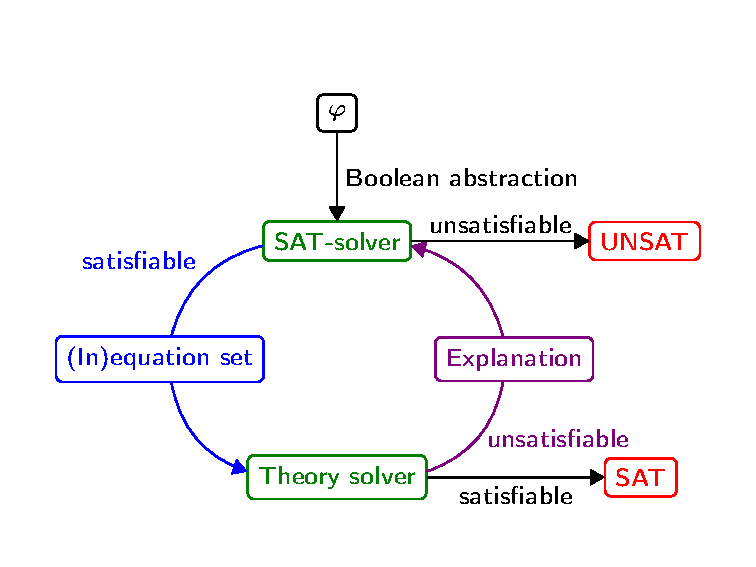
\includegraphics[width=0.7\linewidth]{./figures/FullLazySMT.pdf}
  \caption{Full lazy SMT solver \cite{brahm2010ALS}}
  \label{fig:FullLazySMT}
\end{figure}

%/////////////////////////////////////////////////
%/
\section{Approximation-Based Approach}
%/
%/////////////////////////////////////////////////
\label{sec:Approximation_Based_Approach}
% checked
NRA formula is hard to solve, and the applicability is restricted in practice because the decision procedures are computationally intensive.
That is why we perform linearization for NRA formula.\newline

\noindent Our thesis work is inspired by the Ph.D. thesis work, "Incremental Linearization for Satisfiability and Verification Modulo Nonlinear Arithmetic and Transcendental Functions" \cite{irfan2018incremental}.
The authors of \cite{Cimatti:2018:ILS:3274693.3230639} deal with the problems of SMT and Verification Modulo Theories (VMT), exposes the reachability of first-order modeling provided by SMT solver, over quantifier-free NRA and quantifier-free NRA augmented with transcendental functions (NTA).
Transcendental functions include the exponential function, the logarithm, and the trigonometric functions.\newline

\noindent The main idea of \cite{Cimatti:2018:ILS:3274693.3230639} is to abstract non-linear multiplication and transcendental functions as uninterpreted functions (UFs) as described in Section \ref{subsec:IL_For_SMT} below.
This abstraction is performed iteratively over an abstract domain containing LRA and uninterpreted function.
The uninterpreted functions are used to model non-linear and transcendental functions that are iteratively and incrementally axiomatized with a lemma-on-demand approach \cite{Cimatti:2018:ILS:3274693.3230639}.
In other words, a refinement of the abstraction is performed, and spurious interpretations are eliminated to be closer to satisfying solutions of the formula.
The authors named this abstraction-refinement approach as Incremental Linearization (IL).\newline

% checked
\begin{definition}
    (Uninterpreted Functions).
    The theory of uninterpreted functions (UFs) is the first-order theory with no restriction on the signature $\sum$, the set of non-logical symbols \cite{Cimatti:2018:ILS:3274693.3230639}.
 \end{definition}
 
\noindent Multiplication between variables is abstracted as a binary uninterpreted function.
Detection of spurious models helps to tighten the abstraction.
After detecting the spurious models, for each abstraction-refinement loop, some linear constraints are added to the input formula loop to tighten the abstraction.
The linear constraints include tangent planes resulting from differential calculus and monotonicity constraints \cite{Cimatti:2018:ILS:3274693.3230639}.
On the other hand, each transcendental function is abstracted as a unary uninterpreted function.
Taylor series is used to compute the coefficients.
When spurious models are found, the piecewise-linear axioms are instantiated with upper and lower bound.
For transcendental functions, the abstraction refinement is based on the addition.\newline

% checked
\noindent In \cite{Cimatti:2018:ILS:3274693.3230639}, the authors have explained their contributions for the SMT case briefly and also described the extension of IL from the SMT to the VMT case. 
However, we are only concerned about the details of the refinement mechanisms and of the detection of satisfiable results for SMT case only.
Also, this thesis work does not deal with transcendental functions.
So, we will not be going into the details of the authors' contributions regarding the transcendental functions for SMT case.

\noindent Next we give a brief explanation of solving NRA formulas by IL for SMT case according to \cite{Cimatti:2018:ILS:3274693.3230639}:
%/////////////////////////////////////////////////
%/
\subsection{Incremental Linearization for SMT (NRA)}
%/
%/////////////////////////////////////////////////
\label{subsec:IL_For_SMT}
% checked
Authors have chosen this kind of presentation of the multiplications and transcendental functions for the simplicity of the presentation.
The authors have proposed the Algorithm \ref{alg:IL_For_SMT} for SMT solving on NRA.\newline

\noindent The input is an NRA formula $\varphi$.
The algorithm returns a boolean value if $\varphi$ is detected to be satisfiable or unsatisfiable.
If $\varphi$ is unsatisfiable, it also returns the set of constraints $\Gamma$, a combination of uninterpreted function and LRA (UFLRA).
But if $\varphi$ is satisfiable, it returns the empty set $\emptyset$.\newline

\begin{algorithm}
\caption{The main algorithm SMT-NRA-CHECK \cite{Cimatti:2018:ILS:3274693.3230639}} 
\label{alg:IL_For_SMT}
SMT-NRA-CHECK($\varphi$)
\begin{algorithmic}[1]
\State $\varphi^\prime :=$ SMT-PREPROCESS$(\varphi)$
\State $\hat{\varphi} :=$ SMT-INITIAL-ABSTRACTION$(\varphi^\prime)$
\State $\Gamma := \emptyset$
\While {true}
\State $\langle sat, \hat{\mu} \rangle := $SMT-UFLRA-CHECK$(\hat{\varphi} \wedge \bigwedge \Gamma)$
\State \textbf{if not} sat:
\State $\hspace{5mm} \textbf{return} \hspace{1mm}\langle \textbf{false}, \Gamma \rangle$
\State $\langle sat, \Gamma^\prime \rangle := $CHECK-REFINE$(\varphi, \hat{\varphi}, \hat{\mu})$
\State \textbf{if} sat:
\State $\hspace{5mm} \textbf{return} \hspace{1mm}\langle \textbf{true}, \emptyset \rangle$
\State $\Gamma := \Gamma \cup \Gamma^\prime$
\EndWhile
\end{algorithmic}
\end{algorithm}

% checked
\noindent In line $1$, a method SMT-PREPROCESSOR is invoked which performs a preprocessing step.
This preprocessing step generates  a formula $\varphi^{\prime} = \varphi \wedge \varphi_{shift}$ where $\varphi_{shift}$ defines the values of some fresh real variables $w_{x}$ in terms of some variables $x$ in $\varphi$.
Then in line $2$, the method SMT-INITIAL-ABSTRACTION performs the abstraction of the formula $\varphi^{\prime}$ and then returned an abstracted formula that is assigned to $\hat{\varphi}$.
The abstraction means recursively replacing each non-linear term e.g., $x \ast y$ by an uninterpreted function application $f_{\ast}(x, y)$.
So, authors have only used the uninterpreted function for abstraction.
No abstraction is performed for linear multiplications, e.g., $c \ast x$ where $c$ is a constant, hence all the linear multiplications of $\varphi^{\prime}$ remain unchanged.\newline

\noindent The set of constraints $\Gamma$ is initialized to the empty set $\emptyset$.
Lines $4$ to $11$ is a loop where at each iteration the abstraction is refined by extending the set of UFLRA constraints $\Gamma$ that is responsible for removing the spurious solutions.
The satisfiability checking of the formula $\hat{\varphi} \wedge \bigwedge \Gamma$ is performed by invoking the method SMT-UFLRA-CHECK with the formula $\hat{\varphi} \wedge \bigwedge \Gamma$ as input (line $5$).
The method SMT-UFLRA-CHECK is the SMT solver for UFLRA SMT(UFLRA).
This method returns either $true$ with the current satisfying abstracted model $\hat{\mu}$ or $false$ with the unsatisfiable core is defined as follows:\newline

% checked
\begin{definition}
    (Unsatisfiable Core).
    An unsatisfiable core of an unsatisfiable CNF formula is a subset of the clauses of whose conjunction is unsatisfiable.
 \end{definition}

\noindent The loop breaks if the formula $\hat{\varphi} \wedge \bigwedge \Gamma$ is unsatisfiable, meaning that also the input NRA problem $\varphi$ is unsatisfiable (lines $6$ to $7$).
Otherwise, in line $8$, the method CHECK-REFINE takes as input the formula $\varphi^{\prime}$, the abstracted formula $\hat{\varphi}$, abstract model $\hat{\mu}$ and the precision variable $\epsilon$ and returns either $true$ with empty set $\emptyset$ or $false$ with a non-empty set of UFLRA constraints $\Gamma^{\prime}$.
A detailed explanation of the method CHECK-REFINE is given in the next Section \ref{subsec:Abstraction_Refinement_and_Spuriousness_Check}. 
There is an another loop breaking condition from lines $9$ to $10$.
The algorithm enters the lines $9$ and $10$ if CHECK-REFINE returns $true$ with $\emptyset$ what means that the solution for the abstraction also satisfies the original input NRA formula $\varphi$.
When none of the mentioned loop breaking condition occurs, the non-empty set of UFLRA constraints $\Gamma^{\prime}$ is added to $\Gamma$ at line $11$, and then the next iteration starts.
%/////////////////////////////////////////////////
%/
\subsection{Abstraction Refinement and Spuriousness Check}
%/
%/////////////////////////////////////////////////
\label{subsec:Abstraction_Refinement_and_Spuriousness_Check}
% checked
The authors propose algorithm \ref{alg:Abstraction_Refinement_and_Spuriousness_Check} for checking the spuriousness of the abstract solution and refining the abstraction.
Algorithm \ref{alg:Abstraction_Refinement_and_Spuriousness_Check} shows that the method CHECK-REFINE takes the original NRA formula $\varphi$, the abstracted formula $\hat{\varphi}$ and the abstracted model $\hat{\mu}$ as inputs.
In line $1$, a method CHECK-MODEL is called on $\varphi$ and $\hat{\mu}$ and this method checks if the formula $\varphi$ is satisfied by the model $\hat{\mu}$.
When CHECK-MODEL returns $true$, the algorithm enters to line $2$, and it returns $true$ with empty set $\emptyset$ by terminating the whole process.
The method CHECK-MODEL is described in Section \ref{subsubsec:Spuriousness_Check_ and_Detecting_Satisfiability}.\newline

\begin{algorithm}
\caption{The algorithm CHECK-REFINE \cite{Cimatti:2018:ILS:3274693.3230639}} 
\label{alg:Abstraction_Refinement_and_Spuriousness_Check}
CHECK-REFINE$(\varphi, \hat{\varphi}, \hat{\mu})$
\begin{algorithmic}[1]
\State \textbf{if} CHECK-NRA-MODEL$(\varphi, \hat{\mu})$
\State \hspace{5mm}\textbf{return} $\langle \textbf{true} \rangle$
\State $\Gamma := $ BLOCK-SPURIOUS-PRODUCT-TERMS$(\hat{\varphi}, \hat{\mu})$
\State \textbf{return} $\langle \textbf{false}, \Gamma \rangle$
\end{algorithmic}
\end{algorithm}

\noindent If the algorithm does not enter to line $2$, it means the abstracted model $\hat{\mu}$ is spurious, and it needs to be refined.
A model is spurious means it violates some multiplications in the original NRA formula $\varphi$ \cite{Cimatti:2018:ILS:3274693.3230639}.
 The method  BLOCK-SPURIOUS-PRODUCT-TERMS is invoked at line $3$ to refine the abstract model $\hat{\mu}$.
The method BLOCK-SPURIOUS-PRODUCT-TERMS takes as inputs $\hat{\varphi}$ and $\hat{\mu}$ and returns a set of UFLRA formulas as described in the next Section \ref{subsubsec:Abstraction_Refinement_for_NRA}.
This set of UFLRA formulas are collected into the $\Gamma$ and then returns false with $\Gamma$ in line $4$ which influences the whole process to be continued further and to proceed for next loop (Algorithm \ref{alg:IL_For_SMT}, lines $9$ to $10$).
So, the Algorithm \ref{alg:Abstraction_Refinement_and_Spuriousness_Check} is terminated either the original formula $\varphi$ is found satisfiable, or a set of refinement constraints is being created.\newline

\noindent This was a high-level description of the abstraction refinement and spuriousness check.
We have described the concept of this refinement and spuriousness check-in details in the following Sections \ref{subsubsec:Abstraction_Refinement_for_NRA} and \ref{subsubsec:Spuriousness_Check_ and_Detecting_Satisfiability}, respectively.
%/////////////////////////////////////////////////
%/
\subsubsection{Abstraction Refinement for NRA}
%/
%/////////////////////////////////////////////////
\label{subsubsec:Abstraction_Refinement_for_NRA}
% checked
\begin{sloppypar}
BLOCK-SPURIOUS-PRODUCT-TERMS is the function where the authors of \cite{Cimatti:2018:ILS:3274693.3230639} have explained the refinement of multiplication terms.
To perform the refinement, they have provided some constraint schemata, shown in Figure \ref{fig:Constraint_Schemata_For_Multiplication} which are tautologies in NRA.
These constraint schemata prevent spurious assignments of the abstract model to multiplication terms.
In BLOCK-SPURIOUS-PRODUCT-TERMS method, it is checked whether the values of multiplication terms satisfy the constraint schemata.
Then the method collects all the unsatisfied constraints from the constraints schemata into a list and returns it to the caller method CHECK-REFINE (Algorithm \ref{alg:Abstraction_Refinement_and_Spuriousness_Check}, line $3$).\newline
\end{sloppypar}

\noindent In Figure \ref{fig:Constraint_Schemata_For_Multiplication}, we can see five types of refinement constraints namely Zero, Sign, Commutativity,
Monotonicity and Tangent-plane where $x, x_{i},y, y_{i}$ are variables and $a, b$ are rational values.
It is straightforward to verify that all the constraints are valid formulae in any theory interpreting $f_{\ast}()$ as $\ast$ \cite{Cimatti:2018:ILS:3274693.3230639}.
Each Zero constraint has a single multiplication term, and that is why the authors called the refinements performed by Zero constraints are called single-term refinements.
On the other hand, the refinements performed by Sign, Commutativity and Monotonicity constraints are called double-term refinements as they involve pairs of multiplication terms.
Moreover, Tangent-plane constraints refer to a single multiplication term, and a single point $(a, b)$ and the refinements by these is called tangent-plane refinements.\newline

% checked
\noindent Before explaining different types of refinements in a formal way, that are mentioned above, it is needed to explain the Tangent-plane constraints as it is the interesting part of all refinement constraints, whereas the Zero, Sign, Commutativity and Monotonicity constraints are self-explanatory.
Notice that, Tangent-plane constraints have equality constraints and inequality constraints.
The equality constraints enforce the correct value of  $f_{\ast}(x, y)$ at $x = a$ or $y = b$ and provide multiplication lines.
On the other hand, the inequality constraints provide bound for $f_{\ast}(x, y)$ while $x$ and $y$ are not on multiplication lines.
Figures \ref{fig:Tangent_Plane_Graph}a and \ref{fig:Tangent_Plane_Graph}b illustrate the surface of the uninterpreted funtion $f_{\ast}(x, y) = x \ast y$ and the top view of the surface respectively.
This kind of surface is known in geometry as hyperbolic paraboloid.\newline

\begin{definition}
    (Hyperbolic Paraboloid).
    A hyperbolic paraboloid is a doubly-ruled surface, i.e., for every point on the surface, there are two distinct lines on the surface such that they pass through the point \cite{Cimatti:2018:ILS:3274693.3230639}.
 \end{definition}
 
%  checked
\begin{definition}
\label{def:Tangent Plane}
    (Tangent Plane).
    A tangent plane at apoint ($a, b$) to a bivariate function $f(x, y)$ is defined as:
    $$f(a, b) + \frac{d}{dx} f(a, b) \ast (x-a) + \frac{d}{dx} f(a, b) \ast (y-b).$$
    For multiplication, this yields the tangent plane $a \ast y + b \ast x - a \ast b$.
    \cite{TangentPlane}.
 \end{definition}

\noindent In Figure \ref{fig:Tangent_Plane_Graph} and \ref{fig:Tangent_Plane_Graph}d we can see that at each point on a hyperbolic paraboloid there is a tangent plane to the hyperbolic paraboloid surface as defined in the Definition \ref{def:Tangent Plane}.
Interestingly, the two lines on the surface going through are also in the tangent plane 
In other words, the two projected lines define how the plane cuts the surface.\newpage

\vspace*{50px}
\begin{figure}[ht!]
\begin{subfigure}{.5\textwidth}
  \centering
  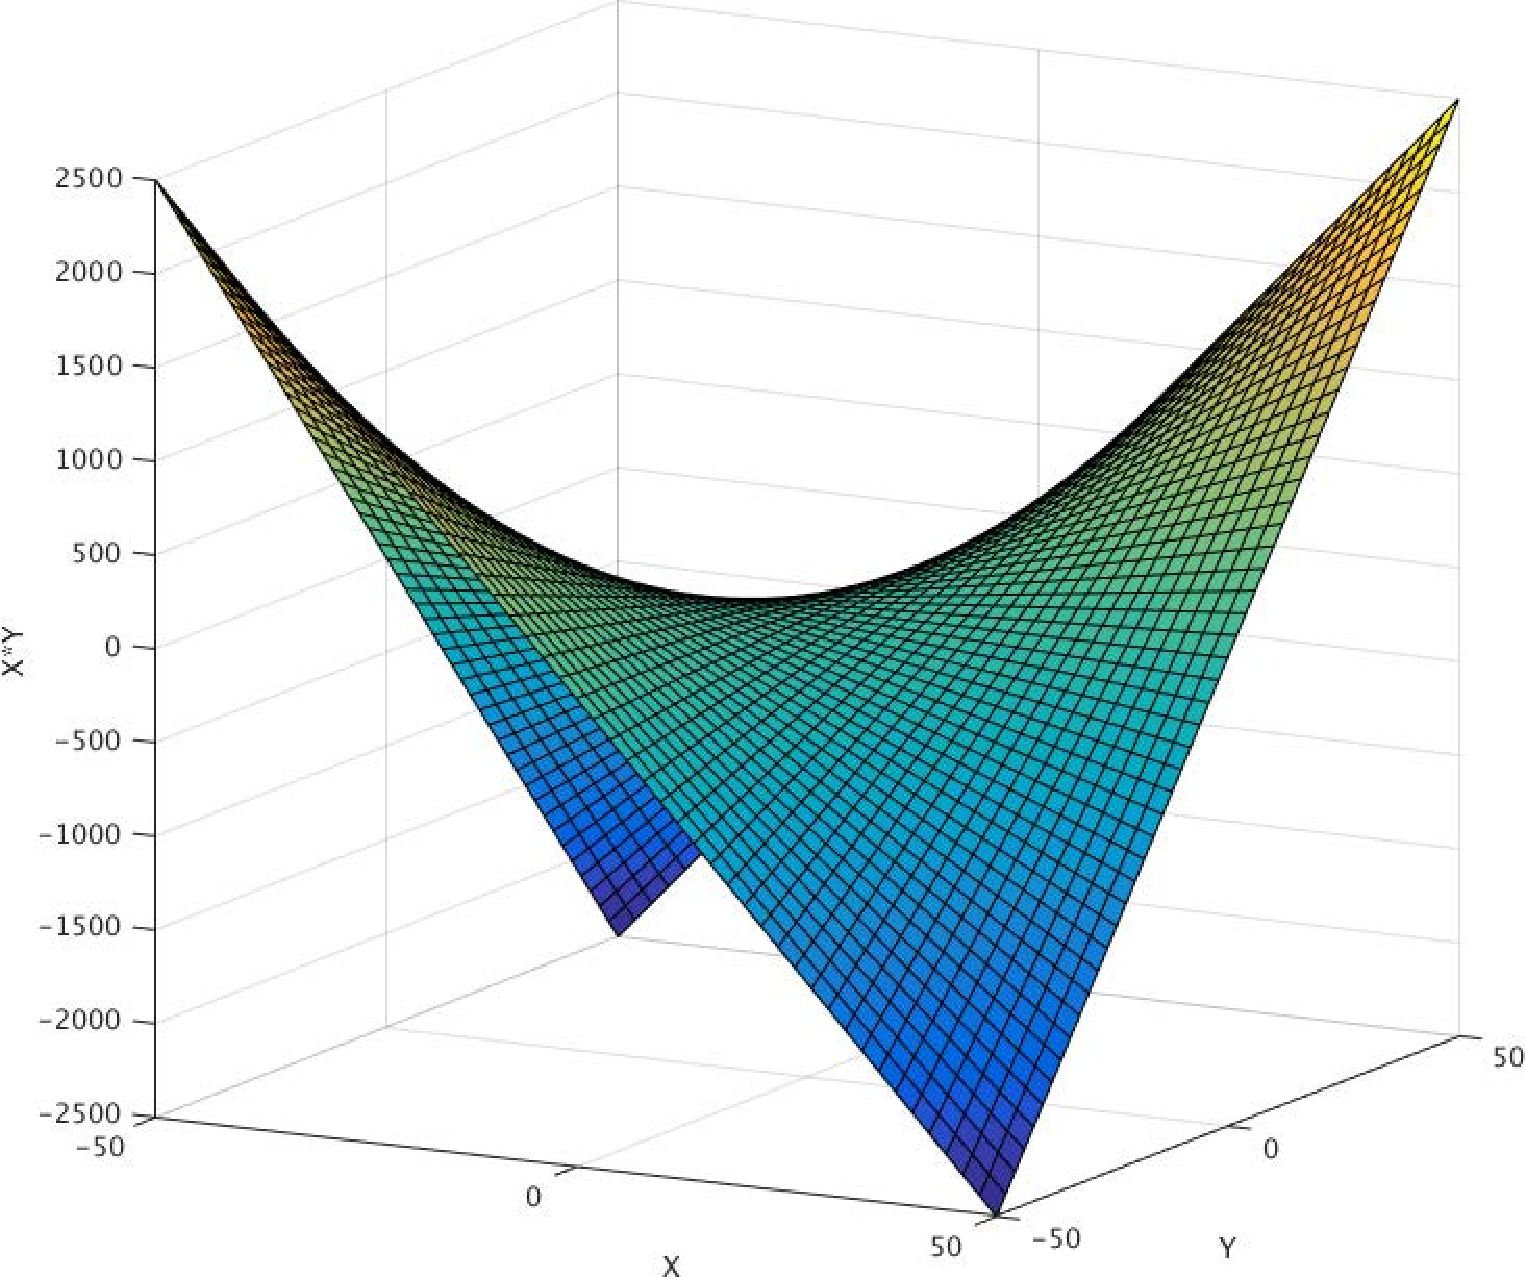
\includegraphics[width=.9\linewidth]{./figures/phdWork_MFunc_a.pdf}
  \caption{$x \ast y$}
  \label{fig:sfig1}
\end{subfigure}%
\begin{subfigure}{.5\textwidth}
  \centering
  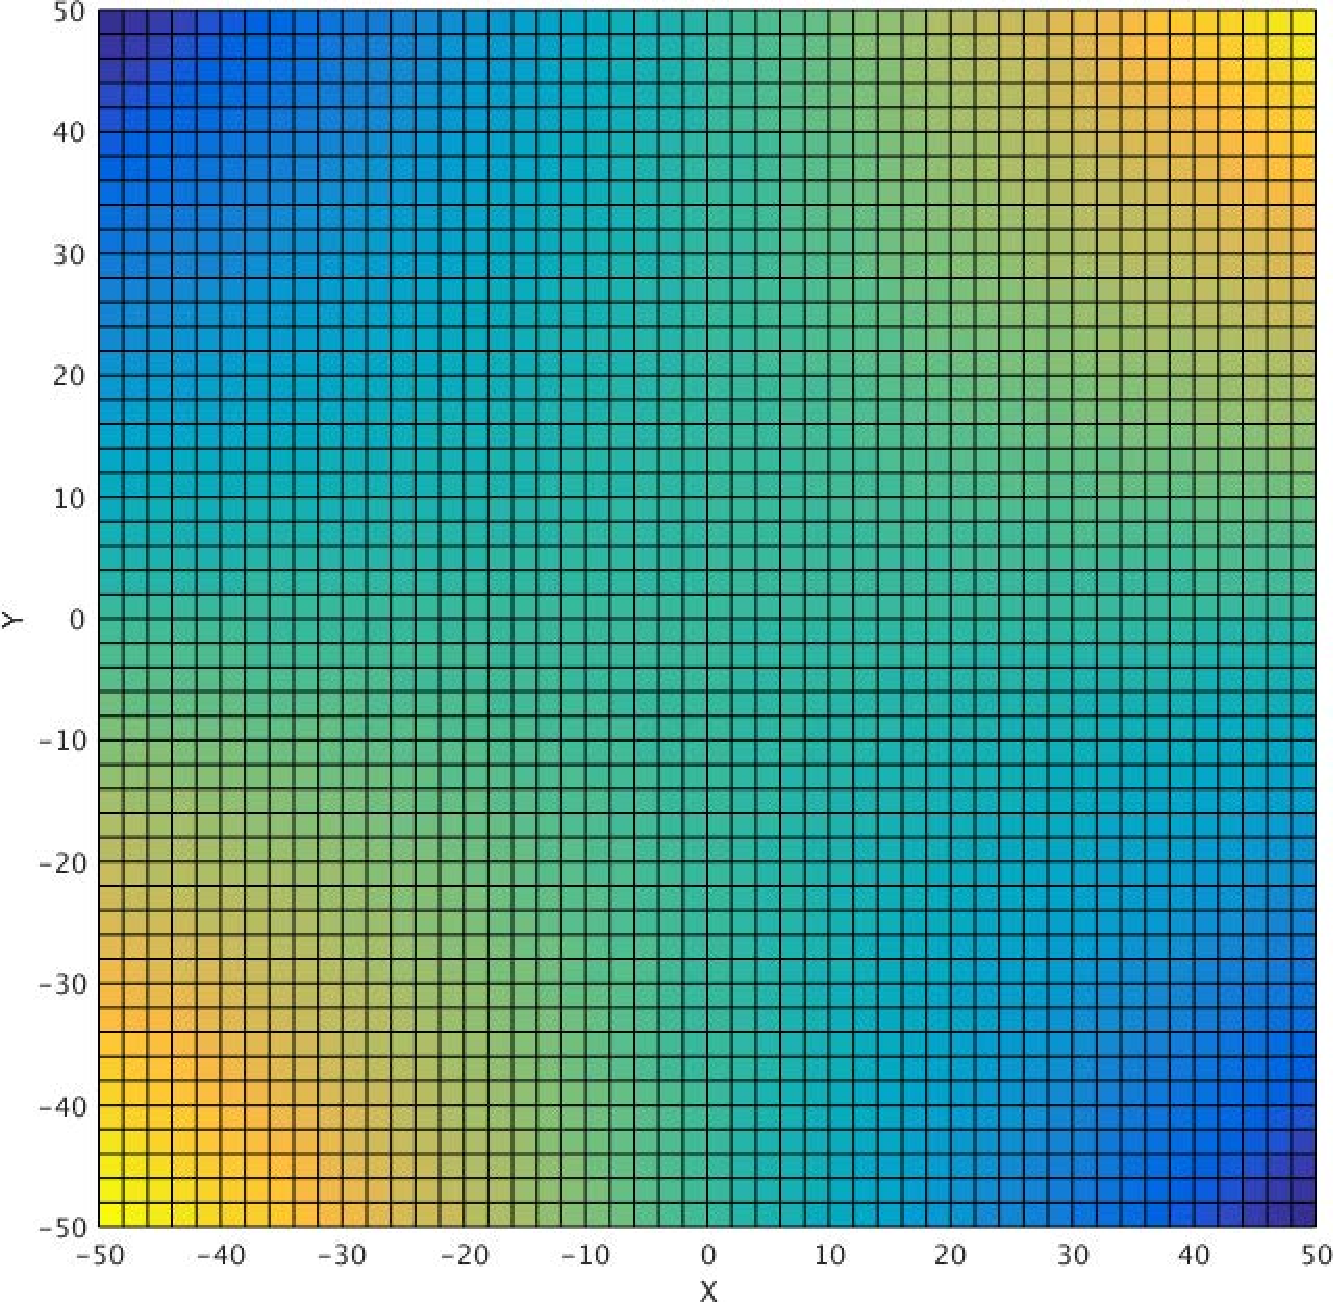
\includegraphics[width=.9\linewidth]{./figures/phdWork_MFunc_b.pdf}
  \caption{$x \ast y$ (top view)}
  \label{fig:sfig2}
\end{subfigure}
\par\bigskip
\par\bigskip
\par\bigskip
\par\bigskip
\par\bigskip
\par\bigskip
\par\bigskip
\begin{subfigure}{.5\textwidth}
  \centering
  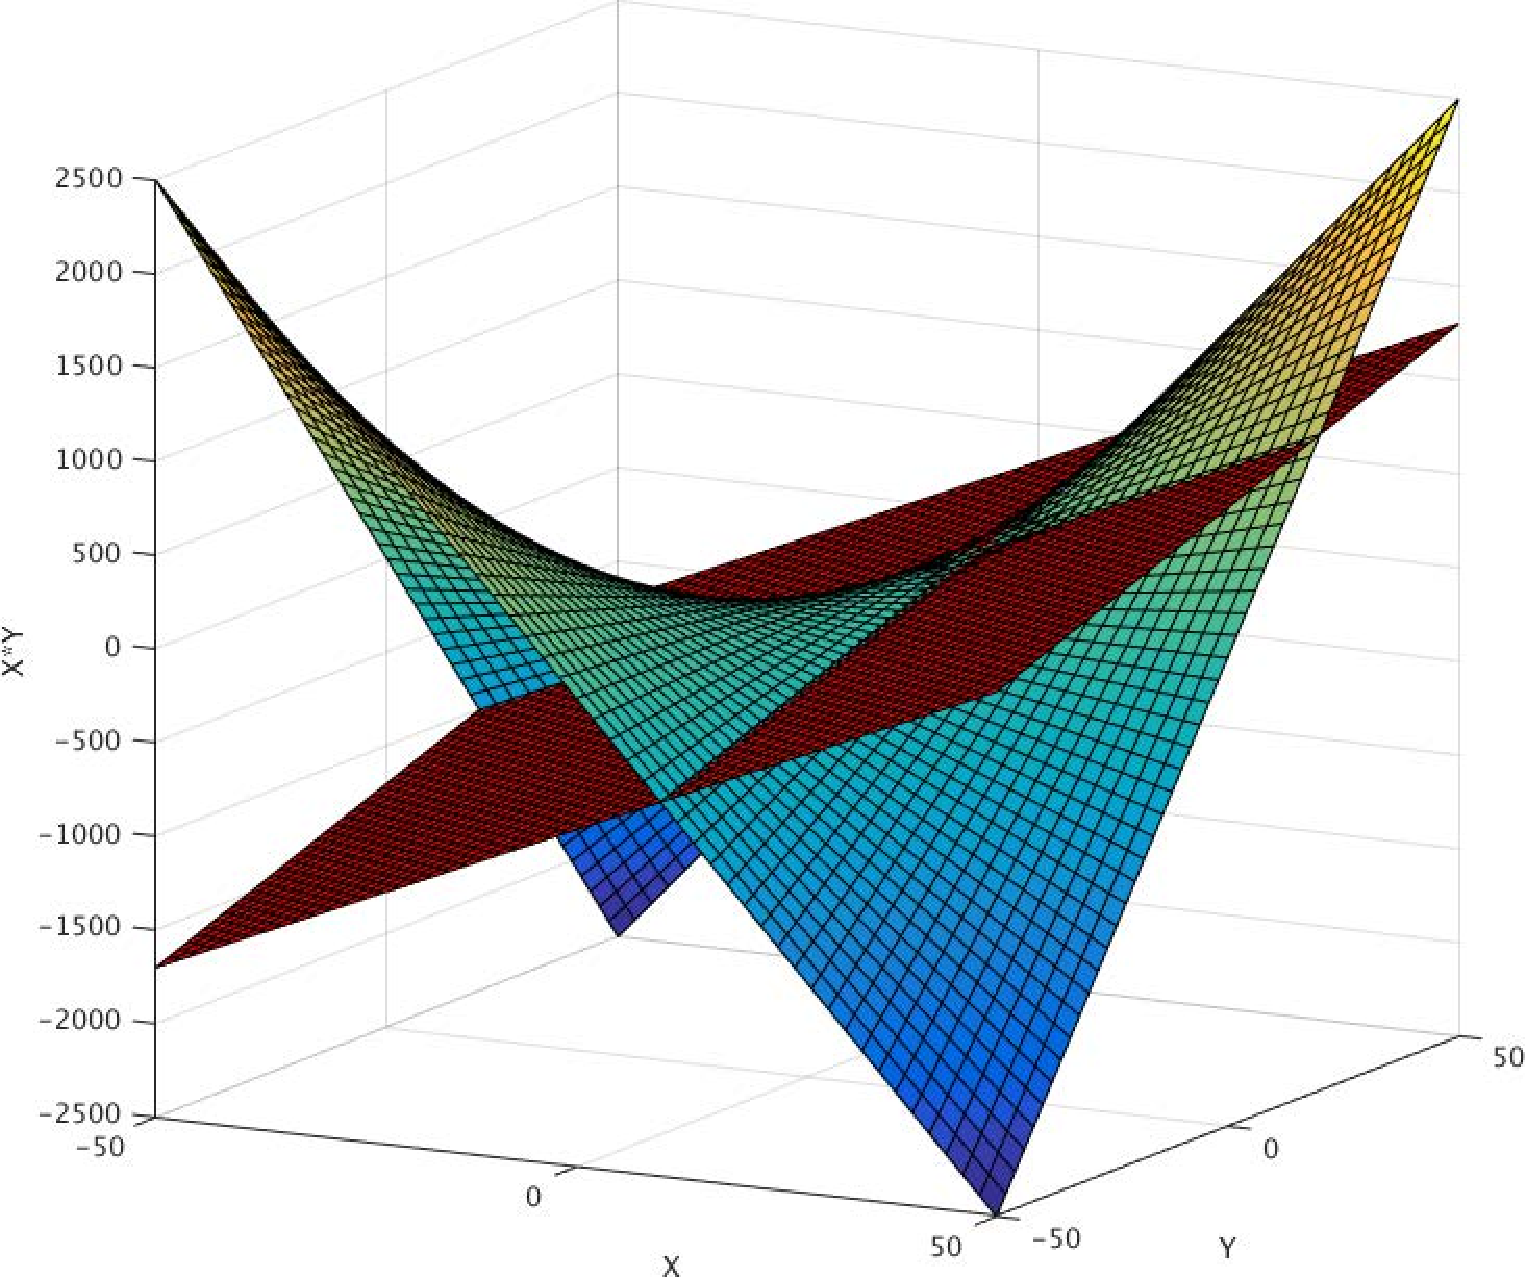
\includegraphics[width=.9\linewidth]{./figures/phdWork_MFunc_c.pdf}
  \caption{$x \ast y$ and tangent plane}
  \label{fig:sfig1}
\end{subfigure}%
\begin{subfigure}{.5\textwidth}
  \centering
  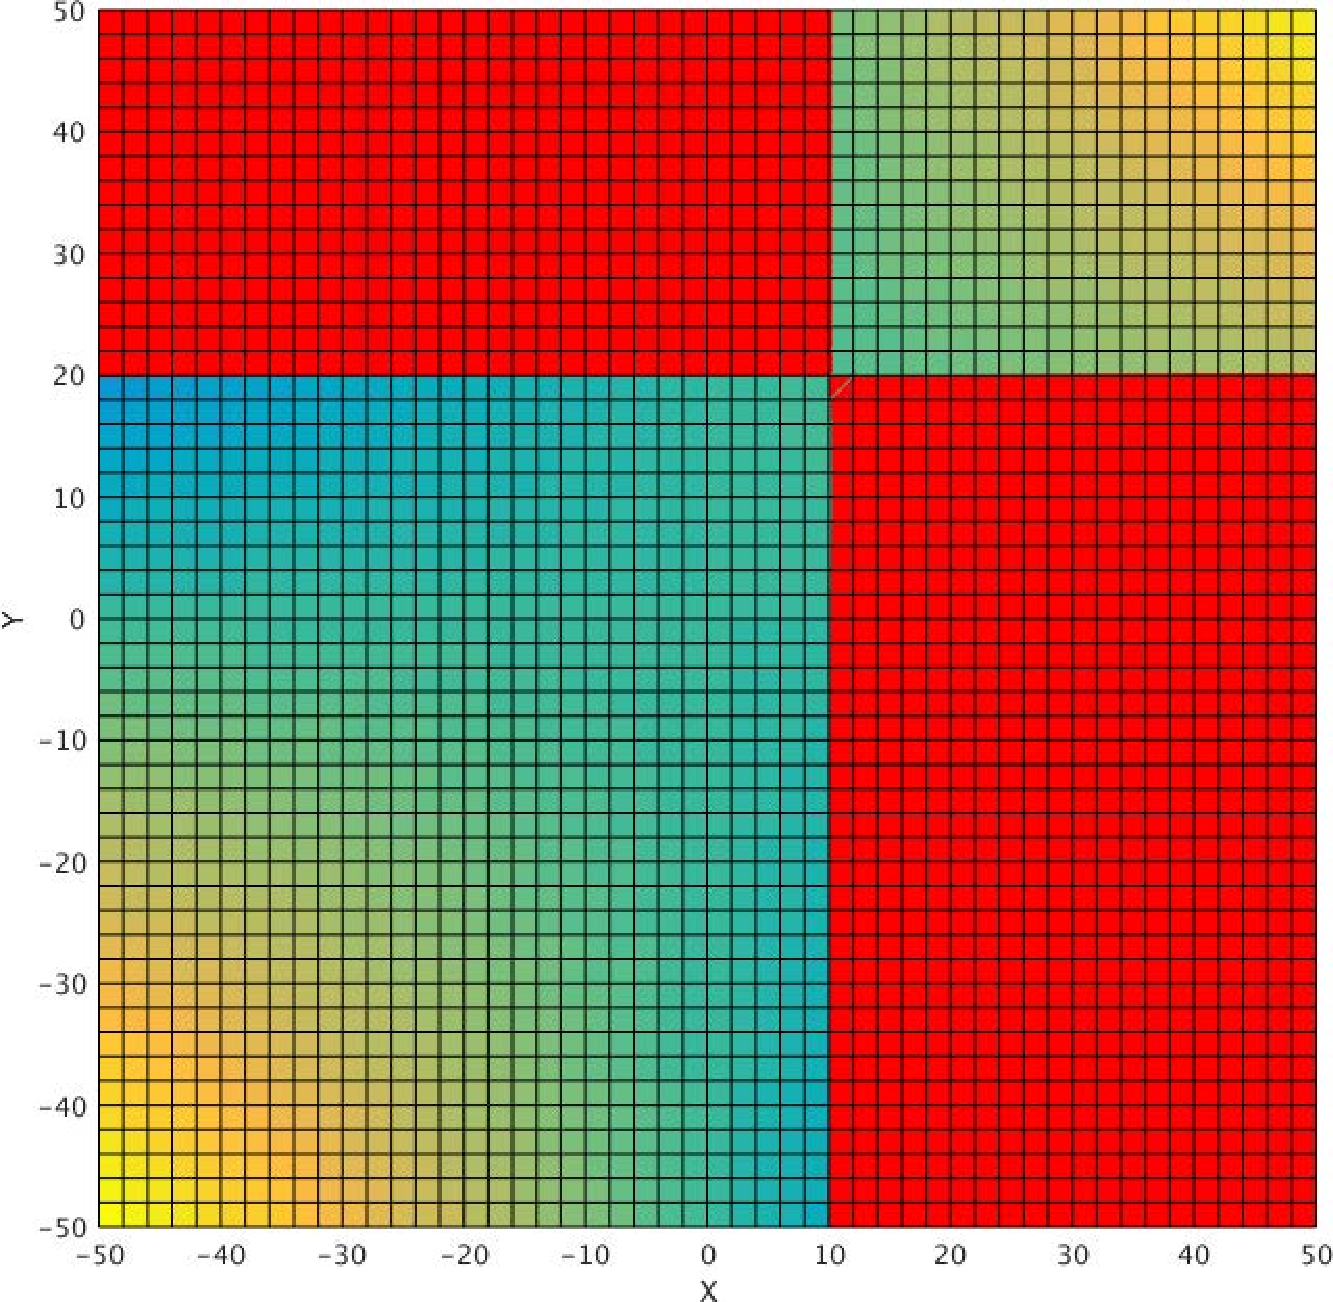
\includegraphics[width=.9\linewidth]{./figures/phdWork_MFunc_d.pdf}
  \caption{$x \ast y$ and tangent plane  (top view)}
  \label{fig:sfig2}
\end{subfigure}
\caption{Multiplication function and tangent plane (these pictures are taken from \cite{Cimatti:2018:ILS:3274693.3230639})}
\label{fig:Tangent_Plane_Graph}
\end{figure}\newpage

\vspace*{40px}
\begin{table}[!ht]
\centering
\def\arraystretch{2.5}
\begin{tabular}{rl}
Zero :          & $\forall x, y. ((x = 0 \vee y = 0) \Leftrightarrow f_{\ast}(x, y) = 0$  \\
               & $\forall x, y. ((x > 0 \wedge y > 0) \vee (x < 0 \wedge y < 0)) \Leftrightarrow f_{\ast}(x, y) > 0$  \\
               & $\forall x, y. ((x < 0 \wedge y > 0) \vee (x > 0 \wedge y < 0)) \Leftrightarrow f_{\ast}(x, y) < 0$  \\
Sign :          & $\forall x, y. f_{\ast}(x, y) = f_{\ast}(-x, -y)$ \\
               & $\forall x, y. f_{\ast}(x, y) = -f_{\ast}(-x, y)$  \\
               & $\forall x, y. f_{\ast}(x, y) = -f_{\ast}(x, -y)$  \\
Commutativity : & $\forall x, y. f_{\ast}(x, y) = f_{\ast}(y, x)$  \\
Monotonicity :  & $\forall x_{1}, y_{1}, x_{2}, y_{2}. ((abs(x_{1}) \leq abs(x_{2})) \wedge (abs(y_{1}) \leq abs(y_{2})) \to$  \\
                & $\hspace{22mm}(abs(f_{\ast}(x_{1}, y_{1}) \leq abs(f_{\ast}(x_{2}, y_{2})))$  \\
                & $\forall x_{1}, y_{1}, x_{2}, y_{2}. ((abs(x_{1}) < abs(x_{2})) \wedge (abs(y_{1}) \leq abs(y_{2})) \wedge (y_{2} \neq 0)) \to$  \\
                &  $\hspace{22mm}(abs(f_{\ast}(x_{1}, y_{1})) < abs(f_{\ast}(x_{2}, y_{2})))$ \\
               & $\forall x_{1}, y_{1}, x_{2}, y_{2}. ((abs(x_{1}) \leq abs(x_{2})) \wedge (abs(y_{1}) < abs(y_{2})) \wedge (x_{2} \neq 0)) \to$ \\
               & $\hspace{22mm}(abs(f_{\ast}(x_{1}, y_{1})) < abs(f_{\ast}(x_{2}, y_{2})))$ \\
Tangent plane : & $\forall x, y. (f_{\ast}(a, y) = a \ast y) \wedge (f_{\ast}(x, b) = x \ast b) \hspace{1mm}\wedge$ \\
               & $\hspace{8mm}((x > a \wedge y < b) \vee (x < a \wedge y > b)) \to f_{\ast}(x, y) < b \ast x + a \ast y - a \ast b \hspace{1mm}\wedge$ \\
               & $\hspace{8mm}((x < a \wedge y < b) \vee (x > a \wedge y > b)) \to f_{\ast}(x, y) >  b \ast x + a \ast y - a \ast b$
\end{tabular}
\end{table}
\begin{figure}[ht!]
\caption{The refinement UFLRA constraint schemata for multiplication \cite{Cimatti:2018:ILS:3274693.3230639}}
\label{fig:Constraint_Schemata_For_Multiplication}
\end{figure}\newpage

\textbf{Different Types of Refinements:}

% checked
\begin{sloppypar}
\begin{itemize}
\item $\textbf{Single-term Refinements:}$
Let us take a constraint schema $\forall x, y. \psi$ from Figure \ref{fig:Constraint_Schemata_For_Multiplication}, containing only one multiplication term i.e., a Zero, Sign, Commutativity or Tangent-plane constraint schema.
For each uninterpreted function application $f_{\ast}(t, s)$ in the abstraction $\hat{\varphi}$, let $\psi^\prime$ results from $\psi$ by replacing $x$ and $y$ by $t$ and $s$, respectively; if this formula evaluates to false under $\hat{\mu}$, then we add $\psi^\prime$ to an initially empty set $ST_{\ast}^{\hat{\mu}}$ of refinement formulas. 
\item $\textbf{Double-term Refinements:}$
Similarly, let us take a constraint schema $\forall x_{1}, y_{1}, x_{2},y_{2}. \psi$ from figure \ref{fig:Constraint_Schemata_For_Multiplication}, containing two multiplication terms i.e., Monotonicity constraint schema.
For each pair of uninterpreted function applications $f_{\ast}(t_{1}, s_{1})$ and $f_{\ast}(t_{2}, s_{2})$, if the formula $\psi^\prime$ that results from $\psi$ by substituting $t_{1}, t_{2}, s_{1}, s_{2}$ for $x_{1}, x_{2}, y_{1}, y_{2}$, respectively, then we add $\psi^\prime$ to $ST_{\ast}^{\hat{\mu}}$.
\end{itemize}
\end{sloppypar}

% checked
\begin{example}
    Consider the input NRA formula $\varphi$ has the multiplication terms $t_{1} \ast s_{1}$ and $t_{2} \ast s_{2}$. These multiplication terms are abstracted by $f_{\ast}(t_{1}, s_{1})$ and $f_{\ast}(t_{2}, s_{2})$, respectively and an abstracted formula $\hat{\varphi}$ is being created.\newline
    
    \noindent Let, $\hat{\mu}$ be an abstract model containing the assignments:
    $$\hat{\mu}[t_{1}] = 2, \hat{\mu}[s_{1}] = 3, \hat{\mu[f_{\ast}(t_{1}, s_{1})]} = 7, \hat{\mu}[t_{2}] = 3, \hat{\mu}[s_{2}] = -4, \hat{\mu[f_{\ast}(t_{2}, s_{2})]} = 5$$
    
    \noindent Then $\hat{\mu}$ violates the third Zero constraint for $t_{2} \ast s_{2}$:
    $$((t_{2} < 0 \wedge s_{2} > 0) \vee (t_{2} > 0 \wedge s_{2} < 0)) \Leftrightarrow f_{\ast}(t_{2}, s_{2}) < 0$$
    
    \noindent The assignment $\hat{\mu}$ does not violate any Sign and Commutativity constraints, but violates all Monotonicity constraints:
    \begin{enumerate}
    \item $((abs(t_{1}) \leq abs(t_{2})) \wedge (abs(s_{1}) \leq abs(s_{2})) \to abs(f_{\ast}(t_{1}, s_{1}) \leq abs(f_{\ast}(t_{2}, s_{2})$
    \item $((abs(t_{1}) < abs(t_{2})) \wedge (abs(s_{1}) \leq abs(s_{2})) \wedge (s_{2} \neq 0) \to (abs(f_{\ast}(t_{1}, s_{1}) < abs(f_{\ast}(t_{2}, s_{2}))$
    \item $((abs(t_{1}) \leq abs(t_{2})) \wedge (abs(s_{1}) < abs(s_{2})) \wedge (t_{2} \neq 0) \to (abs(f_{\ast}(t_{1}, s_{1}) < abs(f_{\ast}(t_{2}, s_{2}))$
    \end{enumerate}
    
    \noindent The assignment $\hat{\mu}$ also violates the Tangent-plane constraint in the points $(2, 3)$ and $(3, -4)$: 
    % (see figure \ref{fig:Tangent_Plane_2_3} and \ref{fig:Tangent_Plane_3_-4}):
    \begin{enumerate}
    \item at the point $(2, 3)$: 
    
    $f_{\ast}(2, s_{1}) = 2 \ast s_{1} \quad \wedge$
    
    $f_{\ast}(t_{1}, 3) = 3 \ast t_{1} \quad \wedge$
    
    $((t_{1} > 2 \wedge s_{1} < 3) \vee (t_{1} < 2 \wedge s_{1} > 3)) \to f_{\ast}(t_{1}, s_{1}) < 3 \ast t_{1} + 2 \ast s_{1} - 6 \quad \wedge$
    
     $((t_{1} < 2 \wedge s_{1} < 3) \vee (t_{1} > 2 \wedge s_{1} > 3)) \to f_{\ast}(t_{1}, s_{1}) > 3 \ast t_{1} + 2 \ast s_{1} - 6$
    \item at the point $(3, -4)$: 
    
    $f_{\ast}(3, s_{2}) = 3 \ast s_{2} \quad \wedge$
    
    $f_{\ast}(t_{2}, -4) = -4 \ast t_{2} \quad \wedge$
    
    $((t_{2} > 3 \wedge s_{2} < -4) \vee (t_{2} < 3 \wedge s_{2} > -4)) \to f_{\ast}(t_{2}, s_{2}) < -4 \ast t_{2} + 3 \ast s_{2} + 12 \quad \wedge$
    
     $((t_{2} < 3 \wedge s_{2} < -4) \vee (t_{2} > 3 \wedge s_{2} > -4)) \to f_{\ast}(t_{2}, s_{2}) > -4 \ast t_{2} + 3 \ast s_{2} + 12$
    \end{enumerate}
    
    \noindent Finally, all these constraints are added to $ST_{\ast}^{\hat{\mu}}$ and returned to refine the abstracted formula $\hat{\varphi}$ which block the spurious model $\hat{\mu}$.
\end{example}

%/////////////////////////////////////////////////
%/
\subsubsection{Spuriousness Check and Detecting Satisfiability}
%/
%/////////////////////////////////////////////////
\label{subsubsec:Spuriousness_Check_ and_Detecting_Satisfiability}
% checked
So far, we have seen how can we perform abstraction refinement by ruling out spurious models.
Now we describe the behavior of the method CHECK-NRA-MODEL.
CHECK-NRA-MODEL is a representation of the method CHECK-MODEL for NRA which detects the satisfiability of the formula $\varphi$ and checks if the model $\hat{\mu}$ is spurious (Algorithm \ref{alg:Check_NRA_Model}).
The authors of \cite{Cimatti:2018:ILS:3274693.3230639} do not want that the algorithm only checks the spuriousness of $\hat{\mu}$, but also detect models, and for that they want the algorithm to look for an actual model for $\varphi$ \enquote{in the surroundings} of $\hat{\mu}$ \cite{Cimatti:2018:ILS:3274693.3230639}, however this procedure of model repair" is not implemented in this thesis and skipped in the following.\newline

\begin{algorithm}
\caption{The algorithm CHECK-NRA-MODEL \cite{Cimatti:2018:ILS:3274693.3230639}} 
\label{alg:Check_NRA_Model}
CHECK-NRA-MODEL $(\varphi, \hat{\mu})$
\begin{algorithmic}[1]
\State $\hat{\psi} := \bigwedge\limits_{A \in T(\varphi, \hat{\mu})} A \quad \wedge \bigwedge\limits_{B \in F(\varphi, \hat{\mu})} B$
\State \textbf{return} $\hat{\mu} \models \psi$
\end{algorithmic}
\end{algorithm}

% checked
\noindent Line $1$ extracts the NRA constraints in $\varphi$ whose linearized abstractions hold under $\hat{\mu}$ \cite{Cimatti:2018:ILS:3274693.3230639}.
Here, $T(\varphi, \hat{\mu})$ contains all atoms in $\varphi$ whose abstraction is $true$ under $\hat{\mu}$ and $F(\varphi, \hat{\mu})$ all those that are $false$ under $\hat{\mu}$.
The algorithm returns whether the NRA concatenations of the abstract constraints have the same truth value, i.e., whether $\hat{\mu}$
 satisfies also $\varphi$.\newline

\noindent The idea of this algorithm is demonstrated by the following example \cite{Cimatti:2018:ILS:3274693.3230639}:\newline

\begin{example}
Consider the following NRA formula $\varphi$ and the abstracted formula $\hat{\varphi}$:
$$\varphi := (x \ast y = 10) \wedge (2 \leq x \leq 4) \wedge (2 \leq y \leq 4)$$
$$\hat{\varphi} := (f_{\ast}(x, y) = 10) \wedge (2 \leq x \leq 4) \wedge (2 \leq y \leq 4)$$

\noindent Assume, SMT-UFLRA-CHECK returns a model $\hat{\mu}$ (Algorithm \ref{alg:IL_For_SMT}, line $5$):
$$\hat{\mu}[x] = 2, \hspace{2mm}\hat{\mu}[y] = 4, \hspace{2mm}\hat{\mu}[f_\ast(x, y)] = 10$$
\end{example}

\noindent So, the method CHECK-REFINE is invoked (Algorithm \ref{alg:IL_For_SMT}, line $8$) and there is still a chance to find a model for the original formula $\varphi$ by using a method CHECK-NRA-MODEL (Algorithm \ref{alg:Abstraction_Refinement_and_Spuriousness_Check}, line $1$ to $2$).
But $2 \hspace{1mm} \ast \hspace{1mm} 4 \neq 10$ and this inequality makes $\hat{\mu}$ spurious and CHECK-NRA-MODEL returns $false$.
